\subsection{Turbopump and Tank Sizing [Drew Sherman]}
With cooling a serious issue in hypersonic aircraft, significant attention must be paid to the coolant used and its conditions. For the regenerative cooling system required by the aircraft’s extreme thermal conditions, it becomes important to understand how the fuel, ethylene, behaves as it cools. One tactic used to ensure predictable and safe cooling is keeping the fuel above its critical point. Ethylene’s critical point is about 5 MPa. Keeping coolant above its critical point theoretically eliminates boiling/two-phase flow concerns as the fuel is pumped over hot material, absorbing heat. The extreme pressure ensures that the liquid will not boil, even in extremely hot environments, which may or may not be seen. Unfortunately, keeping ethylene at this high of a pressure requires a significant initial pressurization and heavy tanks or an active pressurization system on the craft, operating during flight. A simple trade study was used to determine which method should be used to minimize overall system mass. 

It is popular to load the fuel into craft at high pressure, which may be feasible depending on the margin allowed for tank weight. Tank weight is dependent upon the mass and density of the fuel stored and the pressure desired for the fuel in the tank. Standards from ASME \cite{asme} indicate a burst pressure of approximately three times storage pressure, which must be reflected in the weight. According to given conditions, the fuel tanks can achieve a ratio of $PV/W = 1e6 in$. The sizing parameters of the turbopump and listed in table \ref{tab:turboSize}.

\begin{center}
\begin{tabular}{l | c | c}
& Value (SI) & Value (Imperial) \\
\hline
Ethylene Mass & 21 (kg) & 46.3 (lbm) \\
Tank Burst Pressure & 21 (MPa) & 3045 (psi) \\
Ethylene Storage Pressure & 7 (MPa) & 1015 (psi) \\
Ethylene Density & 567.7 (kg/$\text{m}^3$ & 0.02051 (lbm/$\text{in}^3$ \\
Tank Mass & 3.2 (kg) & 6.9 (lbm)
\end{tabular}
\captionof{table}{Turbopump Sizing Parameters}
\label{tab:turboSize}
\end{center}

Initial aircraft sizing and design was based on a small turbopump system that was designed based on parameters from a paper developed by Blank et. all at Purdue University \cite{catalyst}. Figure \ref{fig:turboSchematic} illustrates the major componenets of the turbopump system.

\begin{figure}[H]
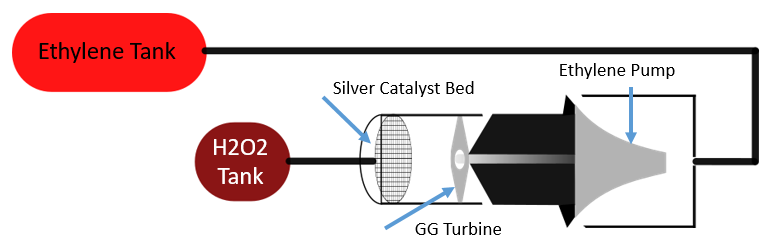
\includegraphics[width=\textwidth]{turboSchematic}
\caption{Turbopump System Illustration}
\label{fig:turboSchematic}
\end{figure}
 
The turbopump is driven by liquid rocket-grade (90\%) hydrogen peroxide (lH2O2) . Sending the peroxide through a silver catalyst bed allows for decomposition and combustion. The products are sent through a small turbine used to drive a pump, raising ethylene pressure. The model is based off catalyst bed loading values and pressure drop values from Blank’s paper \cite{catalyst}. The model uses NASA Chemical Equilibrium Analysis (CEA) to calculate the performance of the silver gas generator at various operating pressures. The rest of the system assumes certain pressure drops, including piping, cooling, and injection pressure losses. Using known and desired conditions for the ethylene, the model solves for the required peroxide massflow to run the pump at various operating pressures by balancing power requirements. Figure \ref{fig:turboPressureVMdot} in Appendix A shows the relationship between gas generator operating pressure and required massflow. 

As can be seen, gas generator chamber pressure affects the amount of peroxide required to drive the pump, but the peroxide massflow is still low. As such, its possible to run the gas generator at low chamber pressures to reduce chances of failure. In addition to solving for massflow, the model generates approximate sizing specifications required for the ethylene pump impeller given assumed performance requirements \cite{sutton}. Given the relatively high performance of the pump, a strong material that can withstand low temperatures and high pressures is required. Research into rocket-grade turbopumps \cite{turbo} shows that RENE 41 should be used for the walls and structure of the gas generator, turbine, and pump assembly due to its high-temperature capability and small thermal expansion[2]. The impeller. since it is estimated at spinning around 30,000 rpm, requires a strong material capable of handling low temperatures. Thus, a titanium alloy containing 5\% aluminum and 2.5\% tin is used, as it is capable of handling the temperature range and intermediate reactive products from the gas generator \cite{sutton}. Sizing and performance characteristics of the gas-generator turbopump system are listed in table \ref{tab:turboParams}. 

\begin{center}
\begin{tabular}{l  c}
Fuel Flowrate (kg/s) & 0.13 \\
$\text{H}_2\text{O}_2$ Flowrate (kg/s) & 0.004 \\
Total $\text{H}_2\text{O}_2$ Mass (kg) & 0.75 \\
Fuel dP (kPa) & 7000 \\
$\text{H}_2\text{O}_2$ Combustion Pressure (kPa) & 345 \\
Impeller Exit Radius (cm) & 6 \\
Impeller Inlet Radius (cm) & 0.5 \\
RPM & 30,000 \\
Wall Material & RENE 41 \\
Iimpeller and Turbine Material & Titanium Alloy \\
Mass (kg) & 5.3 \\
Required Bed Area ($\text{cm}^2$) & 0.15 \\
Bed Loading (lbm/s/$\text{in}^2$) & 0.4 \\
Operating Power (HP) & 3.2
\end{tabular}
\captionof{table}{Turbopump Operational Parameters}
\label{tab:turboParams}
\end{center}

The turbopump system is similarly sized to a typical turbocharger in a car, with higher performance. 

With both pressurization methods analyzed, it becomes obvious that simply storing the ethylene at supercritical pressure results in less mass and less complexity. The turbopump assembly also takes up valuable volume in the center of the craft, which can be used for more fuel to extend range capability. If the required ethylene massflow were to approximately double, the turbopump system begins to show its strengths, especially since tank mass increases linearly with fuel mass. 
 
